% neginhib cogsci submission


\documentclass[10pt,letterpaper]{article}

\usepackage{cogsci}
\usepackage{pslatex}
\usepackage{apacite}
\usepackage{graphicx}

\usepackage{color}
 \newcommand{\denote}[1]{\mbox{ $[\![ #1 ]\!]$}}
 \definecolor{Red}{RGB}{255,0,0}
\newcommand{\red}[1]{\textcolor{Red}{#1}}
\definecolor{Green}{RGB}{10,200,100}
\definecolor{Blue}{RGB}{10,100,200}
\definecolor{DarkOrange}{RGB}{255,100,50}
\newcommand{\ejy}[1]{\textcolor{Blue}{[ejy: #1]}} 
\newcommand{\aen}[1]{\textcolor{DarkOrange}{[aen: #1]}}  
\newcommand{\gabe}[1]{\textcolor{Green}{[gabe: #1]}}  



\title{Distinct mechanisms of linguistic and non-linguistic inference in preschool children}
 
\author{{\large \bf Ann E. Nordmeyer} \\
  \texttt{anordmey@stanford.edu} \\
  Department of Psychology \\
  Stanford University
  \And {\large \bf Erica J. Yoon} \\
  \texttt{ejyoon@stanford.edu} \\
  Department of Psychology \\
  Stanford University
  \And {\large \bf Michael C. Frank} \\
  \texttt{mcfrank@stanford.edu} \\
  Department of Psychology \\
  Stanford University}

\begin{document}

\maketitle


\begin{abstract}

...

\textbf{Keywords:} 
Inhibitory control; negation; implicature; drift diffusion model; cognitive development; pragmatics

\end{abstract}


\section{Introduction}

%
%\ejy{I liked the intro because it's a nice summary of what we're trying to do (so maybe it'll make a good beginning of our abstract) but I wonder if this is still confusing for some naive readers who have no idea what ``linguistic constructions'' we are talking about. I'm going to try something else here (now that I look at it, maybe it won't work... see what you think and feel free to change it back!)}
%
%\aen{I changed it back, because I think it's important to introduce both tasks (and our overarching hypothesis) in the first sentence.  I agree with your overall point, though, and it's something I've been struggling with in this intro because it's hard to introduce so many complicated phenomena so succinctly!  I tried to make it a little clearer what we're talking about here, but I don't know how if this is much better}

Children often fail traditional language processing tasks that test important but complex linguistic constructions.  For example, in tests of negative sentence comprehension, children will often struggle to identify a character who ``doesn't have apples'', instead choosing the character who \emph{does} have apples \cite{nordmeyer2014b}.  And while adults easily make the pragmatic inference that ``My plate has a carrot'' refers to a plate with \emph{just} a carrot rather than a plate with a carrot and a banana, children struggle to make this choice \cite{yoonchildren}.   Although these two examples, negation and pragmatic implicatures, are very different linguistic phenomena, comprehension on both tests requires children to resist choosing a more salient (but incorrect) alternative.  Could poor inhibitory control account for children's difficulty on both of these tasks? 

Children struggle on tasks involving pragmatic implicature: making an inference about a speaker's meaning that goes beyond the literal meaning of an utterance. When people hear a sentence such as ``My friend has glasses'' in a context where there is a person with only glasses and a person with a hat \emph{and} glasses, people assume that the sentence refers to the person with just glasses, because if you had meant the person with a hat you would have said so. Children up to three years of age can struggle to make these contextual implicatures (\citeNP{yoonchildren}, though c.f. \citeNP{stiller2014}) as well as scalar implicatures \cite{huang2009}.  Children's difficulty with these tasks is surprising, because children demonstrate an understanding of pragmatic principles by the age three: children adjust informativeness of their own expressions depending on the difficulty of referent disambiguation \cite{matthews2006} and the extent of listener's knowledge \cite{matthews2012tw}.  

Children's difficulty on another type of test, namely of negation comprehension, is also unexpected given children's early production of negative sentences.  Children spontaneously produce denial negation before their second birthday in both natural \cite{bloom1970, pea1980} and experimental contexts \cite{pea1982}.  Despite this, children as old as four years consistently fail on classic tests of negation comprehension \cite<e.g.>{kim1985, nordmeyer2014b}.  For example, children will look at a picture of a character \emph{with} apples when told to look at the boy with \emph{no} apples, and will rate a puppet's true negative utterance (e.g. ``this is not an apple'', when describing a picture of a banana) as ``silly'' or ``wrong''. If children's production of negative sentences suggests that even two-year-olds have the linguistic knowledge of how negative words work, then children's performance on these tasks may reflect processing difficulties rather than a true lack of comprehension.  

Why do children struggle on these language comprehension tasks when production data and past experiments suggest that they have the requisite linguistic abilities? In both of these examples, children's failures might occur not because they lack linguistic understanding, but because the incorrect choice is more salient or perceptually interesting.  For example, when a child is asked to ``find the boy with \emph{no} apples'', she must look \emph{away} from the character who is holding the labeled objects, and look at some other, unlabeled object instead.  Similarly, to demonstrate comprehension of an ad-hoc implicature, such as ``my plate has a carrot'' referring to a plate with just a carrot instead of a plate with a carrot and a banana, children must look away from the more interesting plate (i.e. the plate with two objects instead of one) to demonstrate understanding of the implicature.  In both of these cases, poor inhibitory control might explain children's difficulty executing the correct response on these comprehension tasks.  Inhibitory control is a broad construct that encompasses a wide variety of different functions \cite{miyake2000} and changes dramatically during early childhood \cite{diamond1996,davidson2006}. We hypothesized that preschool children's poor inhibitory control, rather than undeveloped semantic or pragmatic knowledge, can account for children's failure on negation and implicature comprehension tasks.

\begin{figure*}[!th]
\begin{centering}
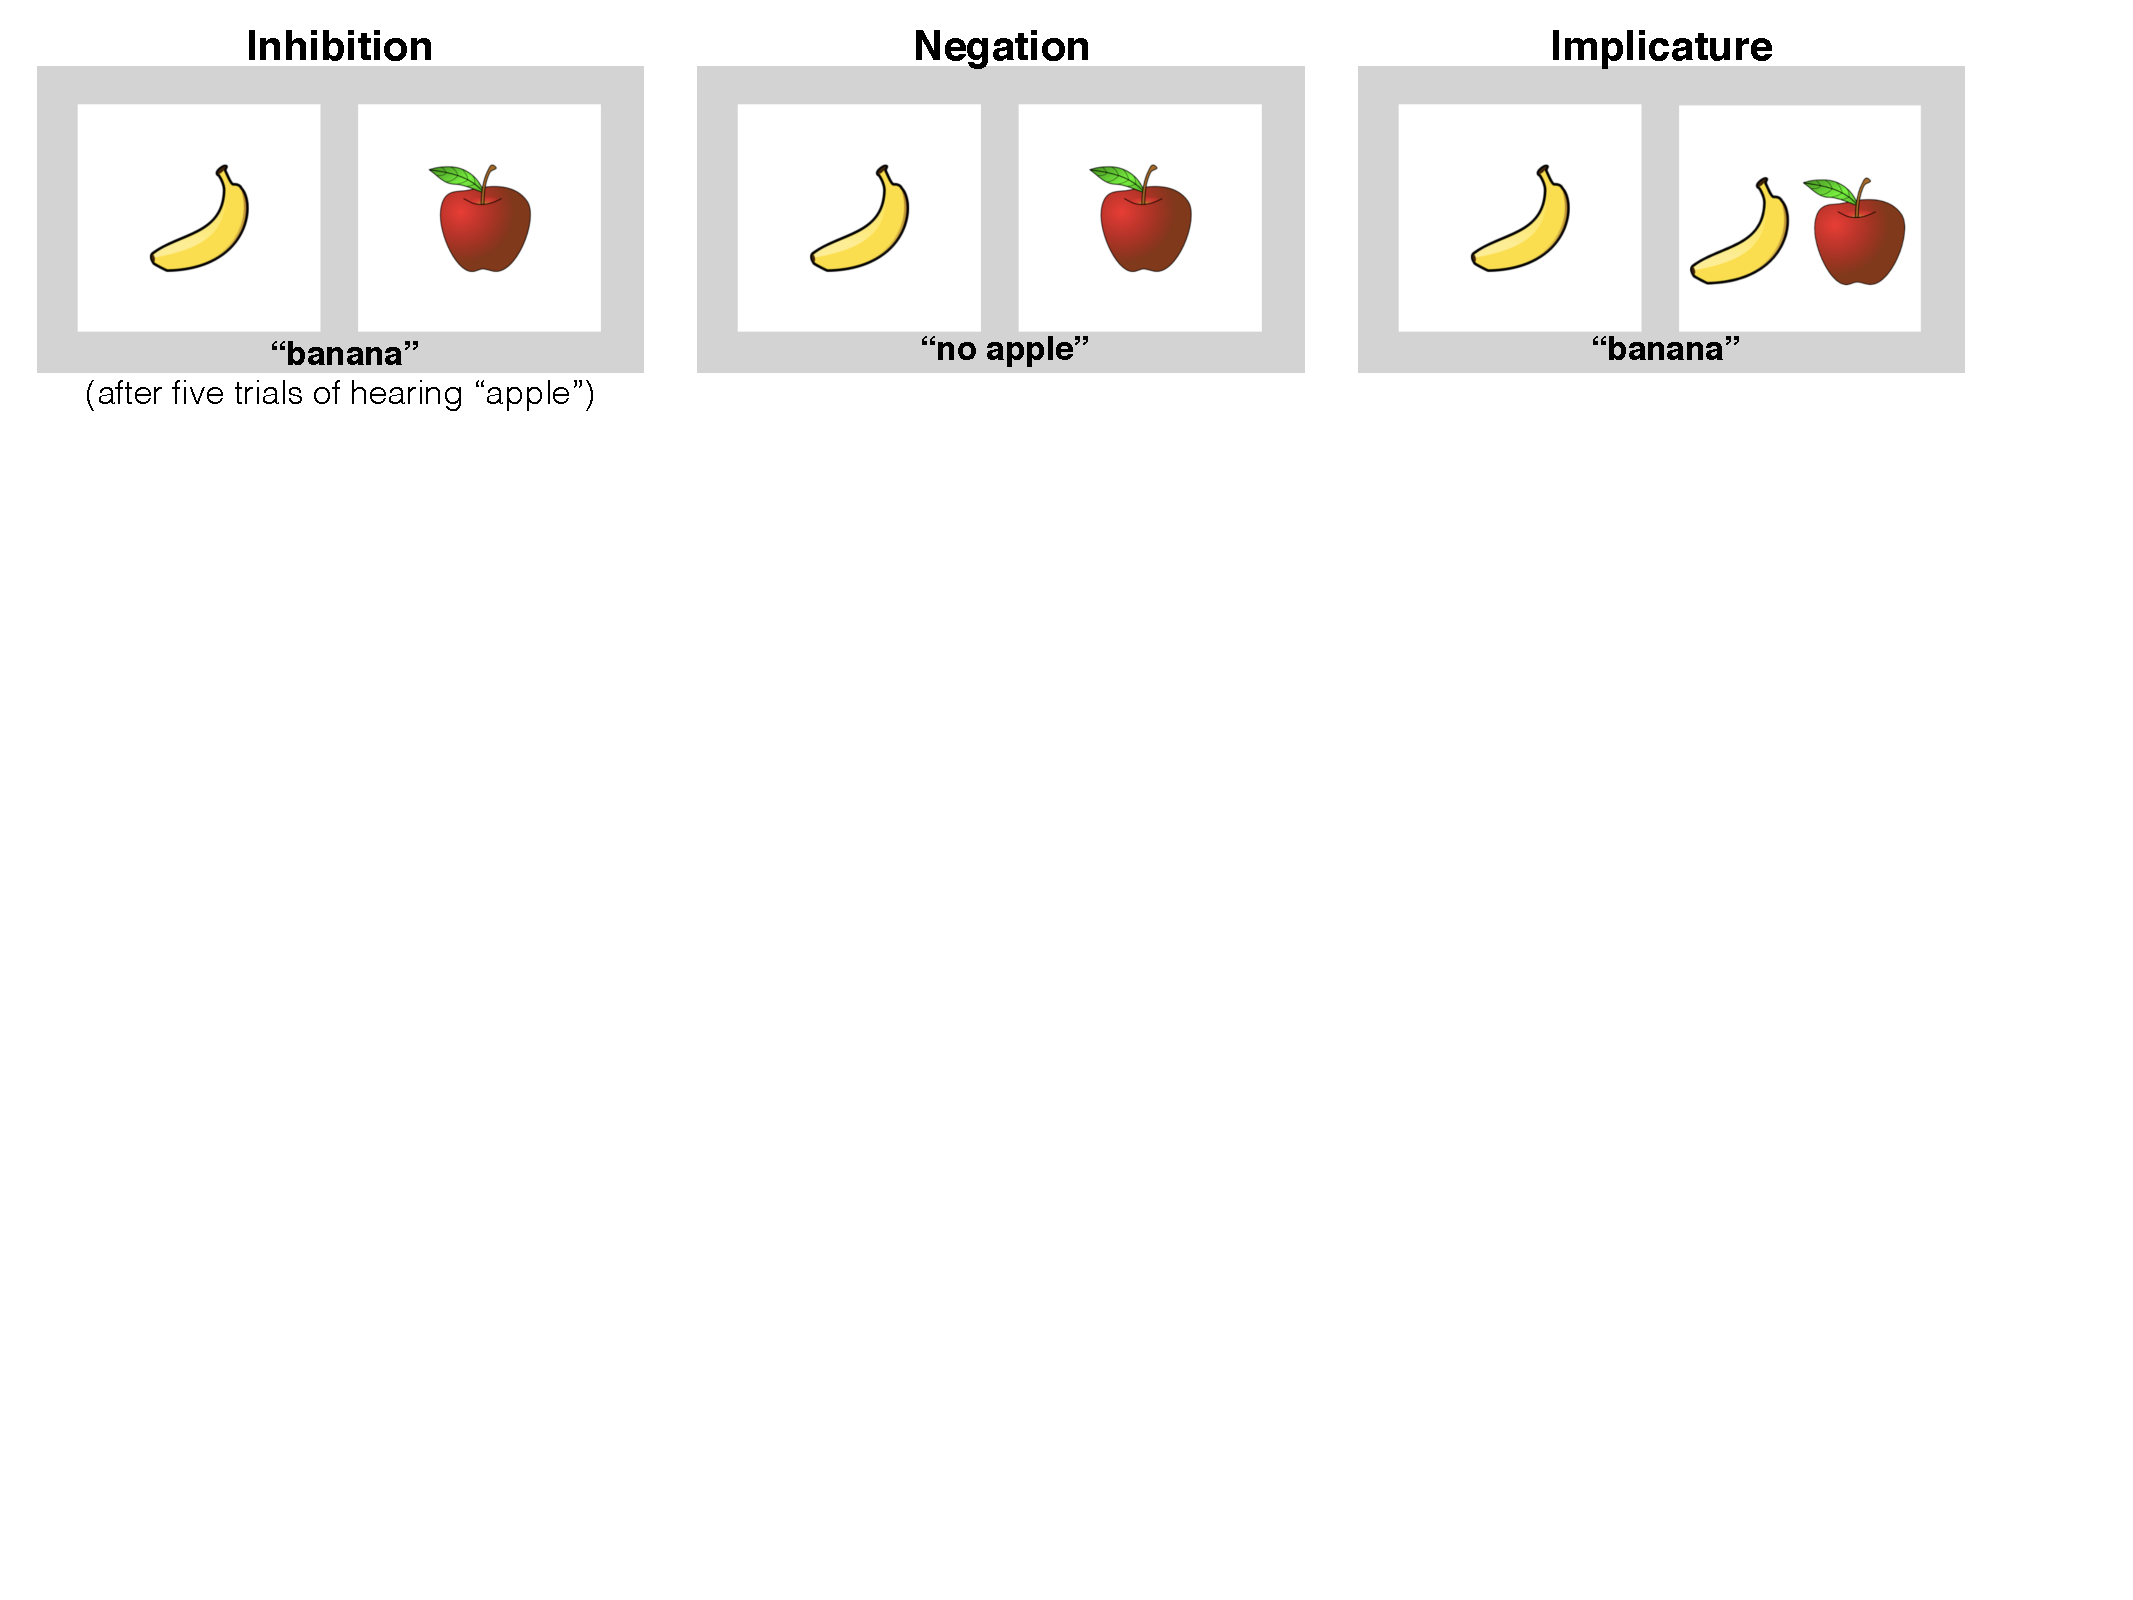
\includegraphics[width=\textwidth]{figures/stimuli.pdf}
\caption{\label{fig:stimuli} Example stimuli from each condition. Words identifying the target picture (left in each panel) are given at the bottom.}
\end{centering}
\end{figure*}

Classic tests of inhibitory control require participants to override a prepotent response. Participants who react quickly often make the wrong choice, and correct choices are typically slower.  This speed-accuracy tradeoff can be difficult to understand with traditional analyses, which examine reaction time and accuracy separately.  
The drift diffusion model \cite<e.g.>{ratcliff1978theory} uses both accuracy and reaction time to model the decision making process in simple two-alternative forced choice paradigms.  The model can be imagined as a noisy accumulation of evidence over time, resulting in an eventual correct or incorrect choice when the accumulated evidence reaches a predetermined ``boundary''.  The model produces four key parameters: boundary separation (the amount of evidence needed to reach a positive decision), bias (to what extent is the decision process biased towards one decision or another), non-decision time (the time needed to encode basic information about the stimuli, before embarking on the decision process), and drift rate (the rate at which evidence is accumulated).  Past work has shown that children typically have longer non-decision times, higher separation boundaries, and slower drift rates, suggesting that children require more time to process stimuli, more information to make a decision, and take longer to accumulate evidence compared to adults \cite{ratcliff2012}. In this study, we use the drift diffusion model to explore whether children's negation and implicature processing resembles their decision-making process on a similar test of inhibitory control.  


In the current study, we use a simple game with three phases to test adults' and children's inhibitory control, negation comprehension, and implicature comprehension.  In order to explore how children's language processing changes across development, we collected data from four-year-olds, five-year-olds, and six-year-olds, as well as adults.  Despite the fact that the three tasks contained almost identical visual and auditory stimuli, we found distinct patterns of information processing and developmental change across the three games.  This suggests that, contrary to our hypothesis, children's poor inhibitory control cannot entirely explain their difficulty with negation and pragmatic implicatures, and children's development of negation and implicature appear to follow different developmental trajectories throughout early childhood. 


\section{Method}

In pilot work, we used a classic ``find the picture'' comprehension task to explore whether 4-year-old children's difficulty processing implicatures and negation might be due to poor inhibitory control.  Our hypothesis was that undeveloped inhibitory control could lead children to quickly choose the more salient incorrect choice rather than selecting the answer they know to be correct.  Although we did not find any correlation between children's inhibitory control processing and their negation or implicature processing, we found that this simple comprehension task was even more challenging for 4-year-olds than our past work has indicated, with 4-year-olds barely exceeding chance performance on negation and implicature trials.  Surprisingly, we found no reaction time differences between 4-year-olds responses to negation/implicature trials and control trials. In our extension of this pilot data we modeled children's responses using the drift diffusion model, which can help us understand the process that leads children to make so many errors on these tasks.  

\subsection{Participants}

We invited parents and children at the Children's Discovery Museum in San Jose, CA to play a computer game.  Ten children whose parents indicated that they hear English at home 50\% of the time or less were excluded from analysis.  An additional 24 children were excluded from analysis for failing to complete at least half of the trials in each game.  This resulted in a final sample of 22 4-year-olds (mean age 4;7), 19 5-year-olds (mean age 5;5), and 25 6-year-olds (mean age 6;5).  We also recruited adult participants (N = 50) on Amazon Mechanical Turk to play the computer version of the task.  Two adults were excluded for failing to complete at least half of the trials in each game, resulting in a final sample of 48 adults.  


\subsection{Stimuli and Design}

The game consisted of three phases that each tested one of the target processes: inhibition, negation processing, and implicature processing.  In each trial in all three phases, there were two images side-by-side on the screen (Figure \ref{fig:stimuli}). A pre-recorded voice said one or two words to refer to one of the images, and participants' task was to select the correct referent as soon as they could identify it. We decided to use words instead of sentences so that we could get fast decisions and many reaction times to accommodate drift diffusion models. 

For the ``inhibition'' phase, in a set of 6-8 trials, the same two pictures appeared side-by-side (e.g., a picture of a banana and a picture of a apple), with randomized sides. For the first 5-7 trials (control trials), one of the two objects was named (e.g., ``apple''), then on the last trial  (target trials), the other object was named (``banana''). Participants were predicted to become increasingly accustomed to choosing the carrot in control trials and thus gain speed. Then in the target trial, when they need to switch and choose the banana, the speed of reaction and accuracy rate were predicted to fall due to the inhibitory demand. Child participants saw a total of 12 sets of trials, and adults saw 24 sets, in the inhibition phase.

For the ``negation'' phase, the referents were named with or without negation. For example, given two pictures of banana and apple respectively, to refer to the banana the recorded voice said ``banana'' (i.e. positive trials, the control for this phase) or ``no apple'' (i.e. negative trials, the target for this phase). Children saw 60 trials, and adults saw 120 trials in the negation phase. 

For the ``implicature'' phase, in each trial there was a picture with one object (e.g., banana) and another picture with the same object and another one (e.g., banana and apple). In control trials, the unique object was named (``apple'') and in target trials, the common object was named (``banana''), implying ``banana \emph{but not apple}'' (i.e. ad-hoc implicature). Children saw 60 trials, and adults saw 120 trials in the implicature phase.  

\subsection{Procedure}

For child participants, an experimenter first explained the game.  Children then went through two practice trials, where they were asked to select an obvious, unambiguous referent (e.g., ``cow'' as opposed to ``rabbit'').  Children selected the picture on the left side of the screen by pressing the `z' key and selected by picture on the right side of the screen by pressing the `/' key; both keys were covered by blue stickers to help children find the correct keys. Then they went through the three test phases in a randomized order.  After the child participants were finished, the experimenter gave them a sticker as a gift and thanked them for playing the game.

Adult participants played the same game without practice trials.  Instructions indicated that participants should select the picture on the right by pressing the `p' key and select the picture on the left by pressing the `q' key.  

\begin{figure}
\begin{center} 
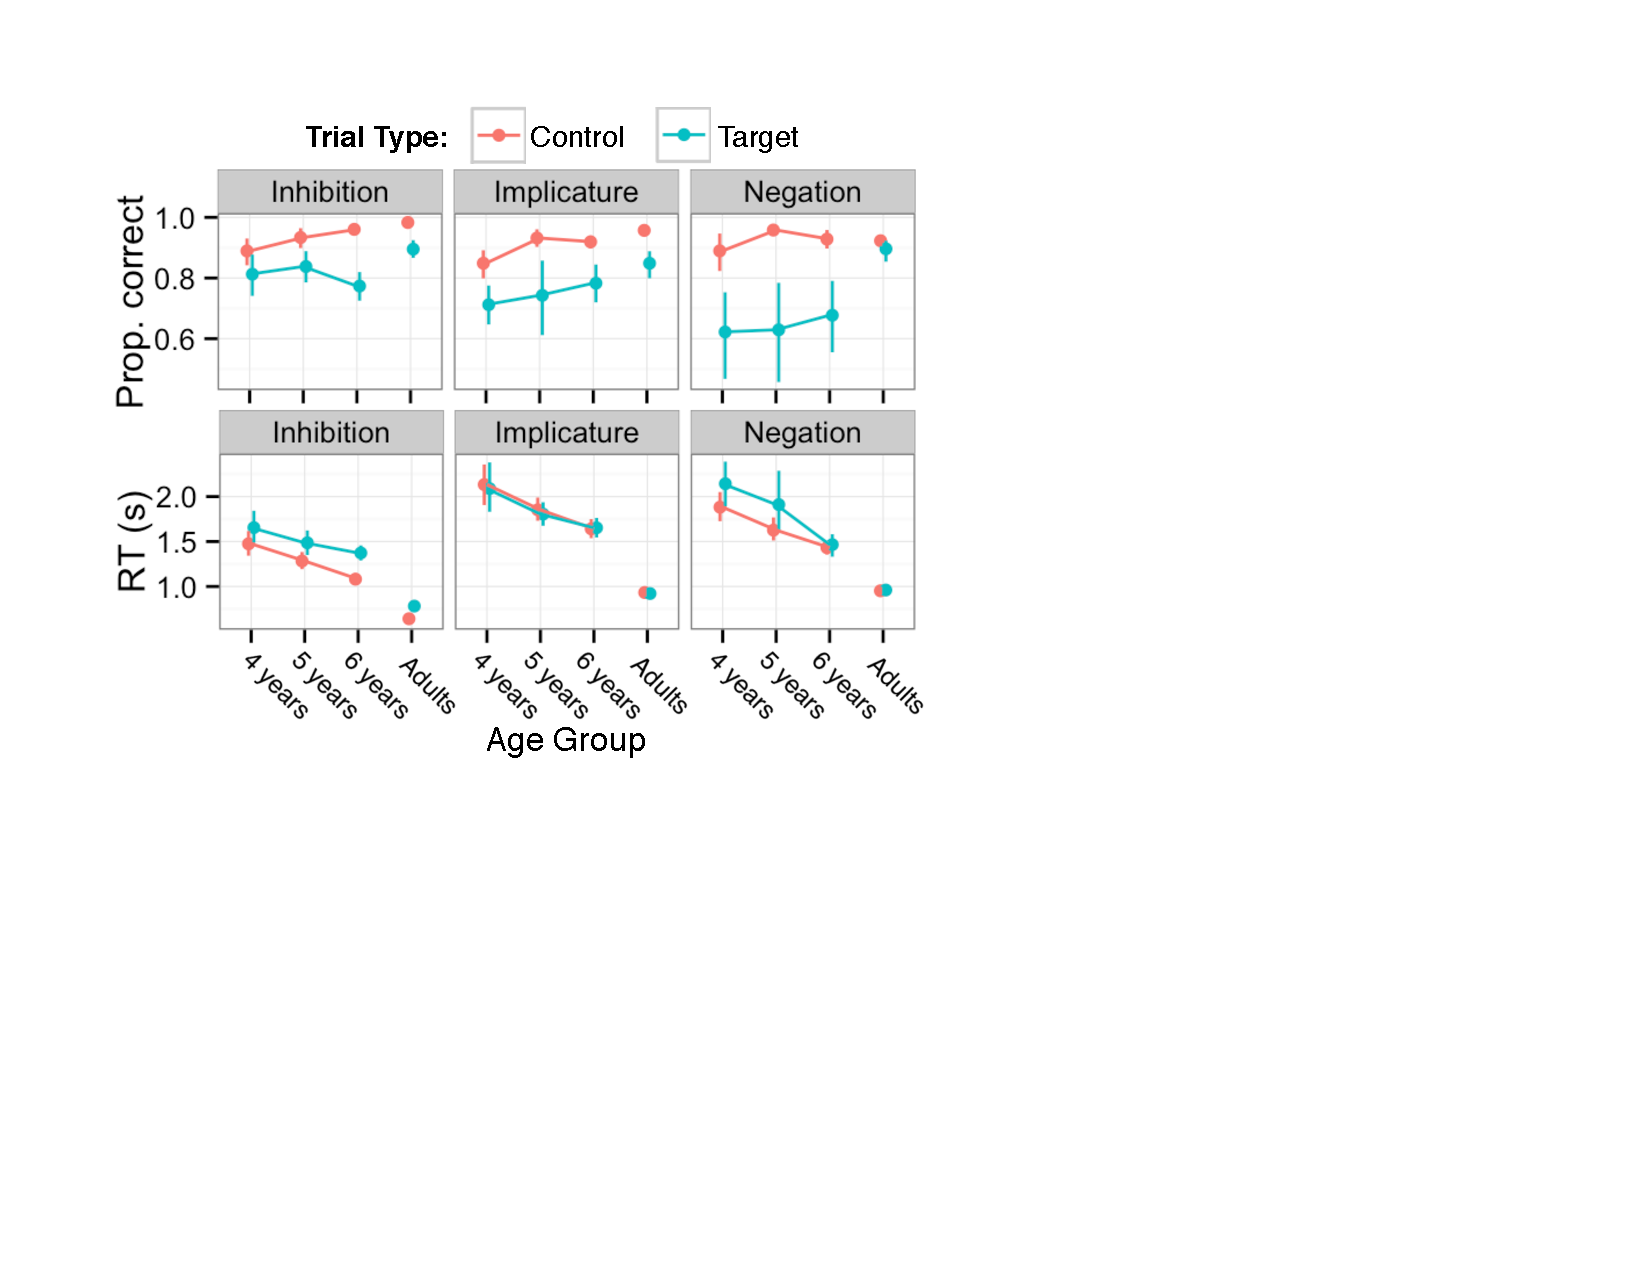
\includegraphics[width=3in]{figures/correct_RT.pdf}
\caption{\label{fig:traditional} Adults' and children's mean proportion correct responses (top) and reaction time (bottom) for target and control trials across the three games.  Control trials are shown in pink, target trials are shown in green.  Error bars show 95\% confidence intervals.  }
\end{center} 
\end{figure}



\section{Results and Discussion}

This experiment yielded a large data set that affords many analyses.  For the sake of this short paper, we focus here on the results that speak most directly to our questions of interest.  Raw data are available at \aen{ADD URL}, and our full set of analyses can be viewed at \aen{ADD URL}.  

For our analyses, because some children responded immediately without listening to the entire word and some children took an exceedingly long time to respond to some trials, we made a post-hoc decision to remove any trials with reaction times less than 200 milliseconds from the word onset, and longer than 15 seconds from the word onset.\footnote{Although this was a post-hoc decision based on some unexpectedly short and long reaction times, this decision did not effect the key findings we present in this paper.}  In addition, in accordance to our planned analysis, we removed any trials where participants responded outside of three standard deviations from the mean in log space.

\subsection{Accuracy and Reaction Time}

\subsubsection{Performance on the inhibition game is not correlated with negation or implicature performance}

We began by looking at participants' accuracy and reaction times on our task (Figure \ref{fig:traditional}).  Across all three games, participants were more accurate on control trials (i.e. repeated trials in the inhibition game, unambiguous trials in the implicature game, and positive trials in the negation game) compared to target trials (i.e. switch trials in the inhibition game, implicature trials in the implicature game, and negative trials in the negation tame).  This difference in accuracy between control and target trials was true across all age groups for the inhibition and implicature games (main effect of trial type in generalized linear mixed-effects model, inhibition game: $\beta = -2.10$, $p< .001$; implicature game: $\beta = -1.145$, $p< .001$); for the negation game, this difference was present for children but not adults (interaction between trial type and age group: $\beta = -1.145$, $p< .001$).  Both children and adults took slightly longer to respond correctly to target trials compared to control trials on the inhibition game (main effect of trial type in linear mixed-effects model, inhibition game: $\beta = 0.140$, $p< .001$), but there was no main effect of trial type in the negation or implicature games.  

Our key hypothesis was that successful performance on the negation and implicature games requires inhibitory control.  To test this, we calculated standardized difference scores between target trial accuracy and control trial accuracy for each participant on each game.  We found no significant correlation between individual accuracy on the inhibition game and the implicature game for adults ($r = .21$, $p = .16$) or kids  ($r = -.07$, $p = .55$), nor did we find a significant correlation between individual accuracy on the inhibition game and the negation game for adults  ($r = -.11$, $p = .46$) or kids  ($r = -.09$, $p = .5$).  

To examine individual differences in reaction time, we calculated standardized difference scores between target trial reaction time and control trial reaction time for each participant on each game.  Again, we found no relationship between individual reaction time on the inhibition game and the implicature game for adults  ($r = .04$, $p = .77$) or kids  ($r = .17$, $p = .18$), nor did we find a relationship between individual reaction time on the inhibition game and the negation game for adults  ($r = .13$, $p = .36$) or kids ($r = -.01$, $p = .95$) \aen{now there's a null correlation!}.  \aen{on a more serious note, I think I could condense this into one paragraph and just say e.g. "none of the correlations were significant" without reporting the exact numbers, what do you guys think?} \ejy{agreed!}.

Consistent with past findings \cite<e.g.>{nordmeyer2014b, yoonchildren}, we found a great deal of individual variability in children's performance on these tasks, with 4- to 6-year-olds struggling especially on the implicature and negation games.  Contrary to our hypothesis, however, children's performance on these two games was not correlated with their performance on the inhibition game.  One drawback to these traditional analyses is that they separate reaction time and accuracy, obscuring any potential interaction between the speed at which participants make a decision and the accuracy of their decision.  In the next section, we fit our data to the Drift Diffusion Model \cite<DDM,>{ratcliff1978theory}, which accounts for both reaction time and accuracy in the decision-making process.  This analysis will allow us to compare participants' information processing in each of these three games across development. 

\subsection{Diffusion Analysis}

We fit the diffusion model separately to each individual participant's data using the RWiener package\footnote{All analyses described in this paper were conducted using R version 3.2.1}, which uses the Nelder-Mead method to estimate optimal parameter values.  We estimated parameters separately for each trial type (target vs. control) within each game, and calculated the mean and 95\% C.I. across all participants within each age group (4-year-olds, 5-year-olds, 6-year-olds, and adults).  We then used these parameter estimates to produce visualizations of the average decision process for each trial type across each game and age group (see Figures \ref{fig:ddm}).  

\subsubsection{Adults show difference decision processes for inhibition, implicature, and negation.}

\begin{figure*}[t!]
\begin{center} 
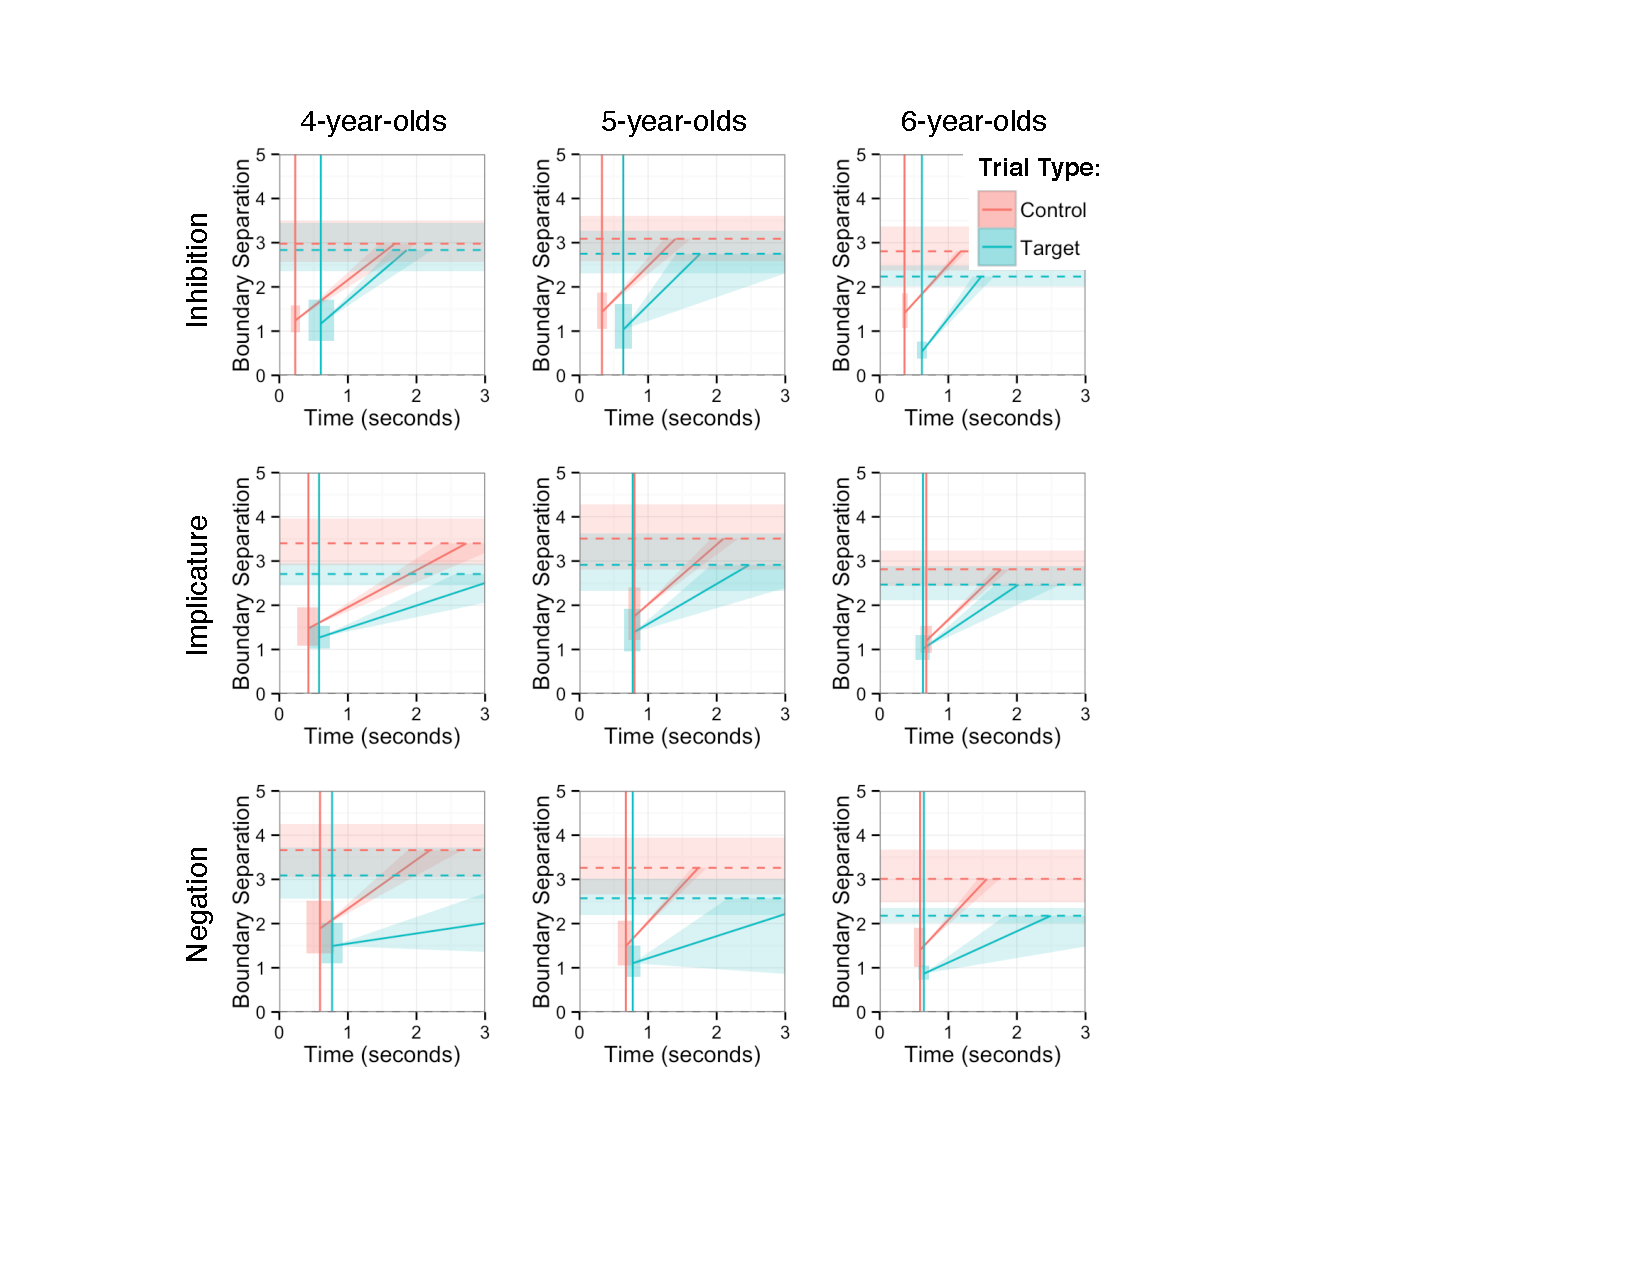
\includegraphics[width=7in]{figures/ddm_vis.pdf}
\caption{\label{fig:ddm} Visualization of the drift diffusion process across the three games.  The process for control trials is shown in pink, and the process for target trials is shown in green.  The dotted black line at zero represents the threshold for making an incorrect decision, and horizontal colored lines represent the boundary separation parameter (i.e. the threshold for making a correct decision).  Vertical colored lines represent the non-decision time parameter, and the slope of the decision process (angled line) represents the drift rate parameters.  The point where the decision process intercepts the non-decision line represents the bias $\times$ boundary separation.  Ribbons around all lines represent 95\% confidence intervals around each parameter.}
\end{center} 
\end{figure*}

First we explored similarities and differences in the decision process for adults across each of the three games (rightmost plots in Figure \ref{fig:ddm}). Surprisingly, despite the surface similarities of these games, the decision process for control vs. target trials appears to be different across the three games.  In the inhibition game, the most striking difference between control and target (inhibition) trials is the bias towards incorrect responses on target trials.  In the implicatures game, the most noticeable difference between control (unambiguous) and target (implicature) trials is the higher boundary separation but faster drift rate for control trials compared to target trials.  In the negation game, there appears to be little difference in the decision process between control (positive) and target (negative) trials.

We conducted post-hoc paired t-tests to compare parameter values for control vs. target trials in each game.  In the inhibition game, the bias parameter was significantly lower (e.g. biased towards the incorrect trial) for target trials compared to control trials ($t(47) = 4.75$, $p< .001$), and target trials had significantly longer non-decision times compared to control trials ($t(47) = -9.36$, $p< .001$).  In the implicature game, the boundary separation and the drift rate were significantly higher for control trials compared to target trials (Boundary Separation: $t(47) = 3.67$, $p< .001$; Drift: $t(47) = 6.64$, $p< .001$).  For the negation game, there was no significant difference between drift rate for control vs. target trials ($t(47) = 1.23$, $p = .23$).  

Although we were surprised by the striking differences across the three games, the decision process that we see makes sense within the context of each game.  For example, we would expect target trials in the inhibition game to be biased towards incorrect responses, because the game is intentionally designed to create such a bias.  The slower drift rate for target trials in the implicatures game might arise due to their ambiguity (i.e. either picture is technically correct), so participants are slower to accumulate information to resolve this ambiguity. The fact that the boundary separation is higher for control trials in the implicatures game, combined with this slower drift rate, explains why reaction times do not differ between trial types on the implicatures game, despite lower accuracy for target trials.  The lack of any difference between positive and negative trials in the negation game was surprising in light of past work suggesting that adults take longer to respond to negative sentences compared to positive ones \cite{hclark1972}, especially in context-free tasks such as this \cite{nordmeyer2014a}.  One possibility is that the high number of repetitive trials, or the simplistic and child-friendly stimuli, made this task easier for adults.

As with the traditional analyses, we found no significant correlations between individual adults' parameters on the different games.\footnote{See \aen{add url} for details on these non-significant correlations}. Next we turned to examining developmental change in children's decision processes, using the DDM to explore general developmental change in children's information processing as well as separate developmental trajectories for each of the three games.

\subsubsection{Children get better at processing information between 4 and 6 years of age.}

First we examined overall changes in children's information processing, regardless of the task that children were engaged in. Across all three games, children at all age groups had higher boundary separation parameters (4-year-olds: $\beta = 1.01$, $p <.001$; 5-year-olds: $\beta = 1.10$, $p <.001$; 6-year-olds: $\beta = .67$, $p <.001$) and longer non-decision times (4-year-olds: $\beta = .08$, $p <.001$; 5-year-olds: $\beta = .19$, $p <.001$; 6-year-olds: $\beta = .11$, $p <.001$) compared to adults, suggesting that children take longer to encode information and need more information to make a decision compared to adults.  Children also had significantly slower drift rates compared to adults (4-year-olds: $\beta = -1.39$, $p <.001$; 5-year-olds $\beta = -1.29$, $p <.001$; 6-year-olds: $\beta = -1.12$, $p <.001$), suggesting that children acquire evidence more slowly than adults.  These data replicate past findings from \citeA{ratcliff2012}, which found similar differences between adults and elementary-school aged children, with a much younger sample of children.  

To explore whether these parameters change significantly throughout these early years, we focused just on children's data and analyzed age group as a continuous variable.  This analysis revealed a significant increase in drift rate across these three years ($\beta = .14$, $p < .05$), as well as a significant decrease in separation bias ($\beta = -.15$, $p < .05$).  These findings indicate that the speed at which children accumulate evidence and the amount of information that children need to make a decision changes rapidly across early childhood.  

\subsubsection{Children show different developmental trajectories in processing implicature and negation.}

Next we examined how children's decision processing changes for each of the three games across development.  In addition to the general developmental change in drift rate, non decision time, and boundary separation described in the previous section, children's decision process for each game shows a distinct pattern of development from four to six years of age.  

\emph{Inhibition:} In the inhibition game, 4-year-olds are actually \emph{less} likely to show a bias towards the incorrect trial compared to adults; this bias appears to get stronger by age 6.  Linear models fit to individual parameter values for each game revealed a significant positive interaction between age group and trial type for four-year-olds' bias parameter ($\beta = .16$, $p< .05$), indicating that for four-year-olds the bias parameter for target trials in the inhibition game is higher compared to adult participants.  There was no interaction between age group and trial type for five-year-olds ($\beta = .07$, $p = .26$), and a marginally significant \emph{negative} interaction between age group and trial type for six-year-olds ($\beta = -.10$, $p = .09$).  These results collectively suggest that while four year olds are \emph{less} biased towards the incorrect response on target trials compared to adults, by age six children are becoming more biased towards the incorrect response on target trials.  

\emph{Implicature:} In the implicature game, children's drift rates increased between four and six years of age, as expected based on our general developmental findings, but this increase in drift rate occurred primarily in control trials.  This led to an increasing difference in drift rates between control and target trials across development, driven primarily by an increase in control trial drift rate.  Drift rates for target trials remain low even in adulthood, presumably due to the ambiguous nature of these trials.  Confirming these findings, linear models fit to individual parameter values for each game resulted in significant positive interactions between age group and trial type at all ages (four-year-olds: $\beta = 0.83$, $p <.01$; five-year-olds: $\beta = 0.71$, $p <.05$; six-year-olds: $\beta = 0.72$, $p <.05$).

\emph{Negation:}  The negation game yielded the most striking difference between adults and children.  Children had strikingly lower drift rates for target trials compared to control trials.  Drift rates on negation trials for four-year-olds were close to zero, suggesting a pattern of general uncertainty for young children on this task.  The primary developmental change for this game was an increase in drift rate for target trials, with significant negative interactions between age group and trial type at all ages (4-year-olds: $\beta = -.7-$, $p <.05$; 5-year-olds: $\beta = -1.00$, $p <.01$; 6-year-olds: $\beta = -.77$, $p <.01$).  

Contrary to our expectations, we found no evidence that children's difficulty on implicature and negation tasks is related to their performance on an inhibitory control task. \ejy{should report on correlations between individual children's parameters somewhere? Or is that going to be in the markdown?}  Furthermore, the drift diffusion analysis yielded informative differences in the development of negation and implicature comprehension.  Although children struggled on both tasks, children's difficulty on the implicature game appears to be due to general changes in information processing across development, as indicated by improvement primarily in the control trials of this game.  In contrast, children's difficulty on the negation game appears to be due to unexpectedly low drift rates for negation trials compared to control trials, a difference that disappears by adulthood.  \emph{Why} children appear to struggle so much on the comprehension of negative sentences, despite producing similar sentences at a much younger age, remains an open question.  


\section{General Discussion}

We designed a game with three similar phases to explore children's and adults' inhibitory control, implicature processing, and negation processing.  Our game was designed to test the hypothesis that negation and implicature processing require inhibitory control, and that children's poor performance on these tasks is due to poor inhibitory control.  Contrary to our hypothesis, we did not find any evidence of a relationship between performance on our inhibition game and performance on the negation or implicature games.  Drift diffusion models revealed strikingly different patterns of processing on all three games, with no evidence that adults or children are biased towards the incorrect answer on implicature or negation tasks.  Our drift diffusion analysis shed light on the developmental trajectory of children's inhibitory control, negation processing, and pragmatic inference, suggesting that children's performance on negation and implicature comprehension tasks may be caused by separate processing difficulties. \aen{is that too strong a claim?} \ejy{I personally think this is nice}

The drift diffusion analysis revealed important findings in our data that could not have been found using traditional analyses of reaction time and accuracy.  Although the three phases of this game were nearly identical in appearance (i.e. using the same few trial images and labels, and the same basic instructions to select the correct picture), the decision process for adults to choose the correct picture was very different for each game.  The inhibition game was characterized by a bias towards the incorrect answer on target trials, for example, while the implicatures game was characterized by slower drift rates for target trials.  

Children's difficulty on these tasks appears to be due to slow accumulation of information, especially for target trials.  Past work suggests that children typically have slower drift rates compared to adults \cite{ratcliff2012}, and our current work replicates that finding in our task.  In our games older children had faster drift rates compared to younger children on all tasks, but this developmental increase in drift rate occurred particularly for control trials on the implicature game \ejy{contradictory to the first sentence of para? ``especially for target trials''} and target trials on the negation game.  The fact that children's drift rates were significantly slower compared to adults for negation trials suggests that children find it particularly difficult to process the relevant information about negation above and beyond a generally slower processing speed for children compared to adults.  Whether the source of this difficulty is an undeveloped semantic understanding of truth-functional negation, or poor phonological processing (e.g. maybe some children simply miss the word ``no''), or some other aspect of executive control, is a topic for future research.  

Another novel aspect of this work is the use of the drift diffusion model with such a young group of children.  Although some past work has explored children's information processing using the drift diffusion model \cite{ratcliff2012}, that work tested second graders at the youngest.  Here we expand on that work by examining a group of even younger children, and replicating their findings.  Our success using the drift diffusion model with data from such young children opens doors for future work exploring the development of children's information processing.

\section{Acknowledgments}
%
We thank the parents, children, and staff at the San Jose Children's Discovery Museum. This work was supported by NSF grant BCS \#1456077. 

%Bing Nursery School, CDM, Stephen Powell, Veronica, Rachel

\bibliographystyle{apacite}

\setlength{\bibleftmargin}{.125in}
\setlength{\bibindent}{-\bibleftmargin}

\bibliography{neginhib}


\end{document}
